\documentclass[12pt,letterpaper]{article}
\usepackage{fullpage}
\usepackage[top=2cm, bottom=4.5cm, left=2.5cm, right=2.5cm]{geometry}
\usepackage{amsmath,amsthm,amsfonts,amssymb,amscd}
\usepackage{lastpage}
\usepackage{enumerate}
\usepackage{fancyhdr}
\usepackage{mathrsfs}
\usepackage{xcolor}
\usepackage{graphicx}
\usepackage{listings}
\usepackage{hyperref}
\usepackage{csvsimple}
\hypersetup{%
  colorlinks=true,
  linkcolor=blue,
  linkbordercolor={0 0 1}
}

\lstdefinestyle{Python}{
    language        = Python,
    frame           = lines, 
    basicstyle      = \footnotesize,
    keywordstyle    = \color{blue},
    stringstyle     = \color{green},
    commentstyle    = \color{red}\ttfamily
}

\setlength{\parindent}{0.0in}
\setlength{\parskip}{0.05in}

\newcommand\course{[F21] DE}
\newcommand\hwnumber{1}
\newcommand\NetIDa{a.korshuk@innopolis.university}
\newcommand\NetIDb{Aliaksei Korshuk}

\pagestyle{fancyplain}
\headheight 35pt
\lhead{\NetIDa}
\lhead{\NetIDa\\\NetIDb\\}
\chead{\textbf{ \Large \\Computational Practicum }}
\rhead{\course \\ \today \\}
\lfoot{}
\cfoot{}
\rfoot{\small\thepage}
\headsep 1.5em

\begin{document}

\begin{center}
    \section*{Source code}
\end{center}

GitHub repository is available \href{https://github.com/AlekseyKorshuk/numerical-methods}{here}.

\begin{center}
    \section*{Exact solution}
\end{center}

Initial value problem:
\begin{equation}
     y'(x) = \frac {\sqrt {y - x}}{\sqrt{x}} + 1
\end{equation}
\begin{equation}
     y(1) = 10
\end{equation}


Solve $ \frac{dy(x)}{ dx} = \frac {\sqrt{-x + y(x)}}{ \sqrt{x}} + 1$, such that $y(1) = 10$:

Let $ y(x) = xv(x)$ , which gives $ \frac{dy(x)}{dx} = x \frac{ dv(x)}{ dx} + v(x)$:
\begin{equation}
     x \frac{ dv(x)}{ dx} + v(x) = \frac{\sqrt{-x + x v(x)}}{\sqrt{x}} + 1
\end{equation}

Simplify:
\begin{equation}
     x \frac{ dv(x)}{ dx} + v(x) = \sqrt{v(x) - 1} + 1
\end{equation}

Solve for $\frac{dv(x)}{dx}$:
\begin{equation}
     x \frac{ dv(x)}{ dx} + v(x) = \sqrt{v(x) - 1} + 1
\end{equation}

\begin{equation}
     \frac{ dv(x)}{ dx} = \frac{ \sqrt{v(x) - 1} - v(x) + 1}{x}
\end{equation}

Divide both sides by $\sqrt{v(x) - 1} - v(x) + 1$:
\begin{equation}
     \frac{\frac{ dv(x)}{ dx}}{\sqrt{v(x) - 1} - v(x) + 1} = \frac{1}{x}
\end{equation}

Integrate both sides with respect to x:
\begin{equation}
    \int {
    \frac{\frac{ dv(x)}{ dx}}{\sqrt{v(x) - 1} - v(x) + 1}
    }dx = \int {\frac{1}{x}}dx
\end{equation}

Evaluate the integrals, where $c_1$ is an arbitrary constant:
\begin{equation}
     -2\log (-\sqrt{v(x) - 1} + 1) = \log (x) + c_1
\end{equation}

Solve for v(x):
\begin{equation}
     v(x) = - \frac{2e^{-\frac{c_1}{2}}}{\sqrt{x}} + \frac{e^{-c_1}}{x} + 2
\end{equation}

Simplify the arbitrary constants:
\begin{equation}
     v(x) = - \frac{2}{c_1\sqrt{x}} + \frac{1}{c_1^2x} + 2
\end{equation}

Substitute back for $y(x) = x v(x)$:
\begin{equation}
     y(x) = x(- \frac{2}{c_1\sqrt{x}} + \frac{1}{c_1^2x} + 2)
\end{equation}

Solve for $c_1$ using the initial conditions:

Substitute $y(1) = 10$ into $y(x) = x(- \frac{2}{c_1\sqrt{x}} + \frac{1}{c_1^2x} + 2)$:
\begin{equation}
     -\frac{2}{c_1} + \frac{1}{c_1^2} + 2 = 10
\end{equation}

Solve the equation:
\begin{equation}
     c_1 = -\frac{1}{2} \text{ or } c_1 = \frac{1}{4}
\end{equation}

Substitute $c_1 = -\frac{1}{2}$ into $y(x) = x(- \frac{2}{c_1\sqrt{x}} + \frac{1}{c_1^2x} + 2)$:
\begin{equation}
     y(x) = 2 (2 \sqrt{x} + x + 2)
\end{equation}

Substitute $c_1 = \frac{1}{4}$ into $y(x) = x(- \frac{2}{c_1\sqrt{x}} + \frac{1}{c_1^2x} + 2)$:
\begin{equation}
     y(x) = 2 (-4 \sqrt{x} + x + 8)
\end{equation}

After collecting solutions the answer is:
\begin{itemize}
    \item
         $y(x) = 2 (2 \sqrt{x} + x + 2)$
    \item
         $y(x) = 2 (-4 \sqrt{x} + x + 8)$
\end{itemize}
Results are continuous on their domain.

\begin{center}
    \section*{How does it work?}
    \subsection*{Input parameters}
\end{center}


\begin{itemize}
    \item
         Function $y$: $y = f(x)$
    \item
         Function $y'$: $y' = f(x,y)$
    \item
         Range of x: $x \in (x_0, X)$
    \item
         Initial solution $y_0$: $y(x_0) = y_0$
    \item
         Range of $n$: $n \in (n_0, N)$
    \item
         Coefficient $c$: one of two possible coefficients after solving initial value problem
\end{itemize}

\begin{center}
    \section*{Sample results}
    \subsection*{Input parameters}
\end{center}

\begin{itemize}
    \item
         Function $y$: $y = x(\frac{-2}{\sqrt{x}c} + \frac{1}{xc^2} + 2)$
    \item
         Function $y'$: $y' = \frac{\sqrt{y - x}}{\sqrt{x}} + 1$
    \item
         Range of x: $x \in (1, 15)$
    \item
         Initial solution $y_0$: $y(1) = 10$
    \item
         Range of $n$: $n \in (2, 15)$
\end{itemize}

\begin{center}
    \subsection*{Graphs}
\end{center}

    \begin{figure}[!h]
    \begin{center}
            \subsubsection*{Exact and numerical solutions}
        \end{center}
        \centering
            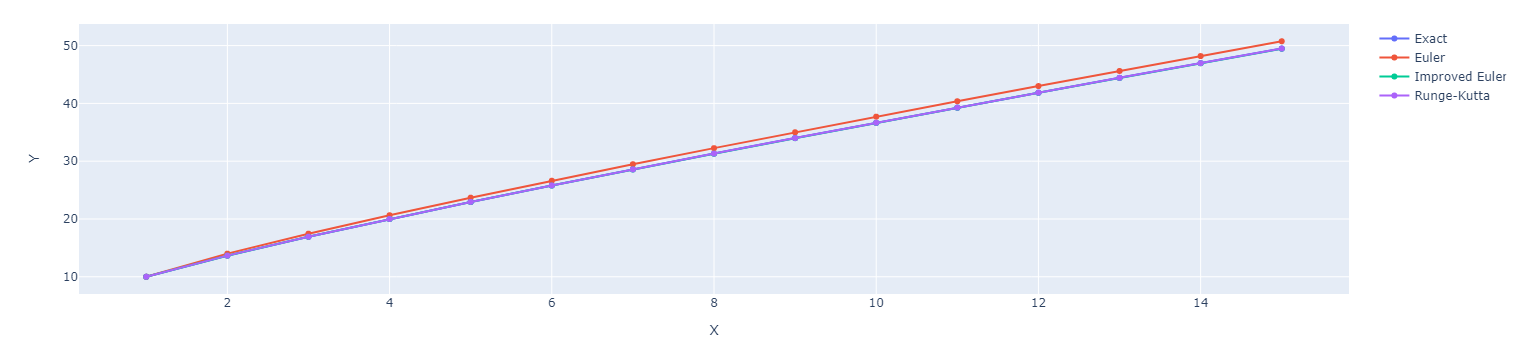
\includegraphics[width=1\linewidth]{solutions.png}
        % \caption{Graph of exact and numerical solutions}
    \end{figure}


\begin{figure}[!h]
    \begin{center}
        \subsubsection*{Total approximation error depending on the number of grid cells}
    \end{center}
    \centering
        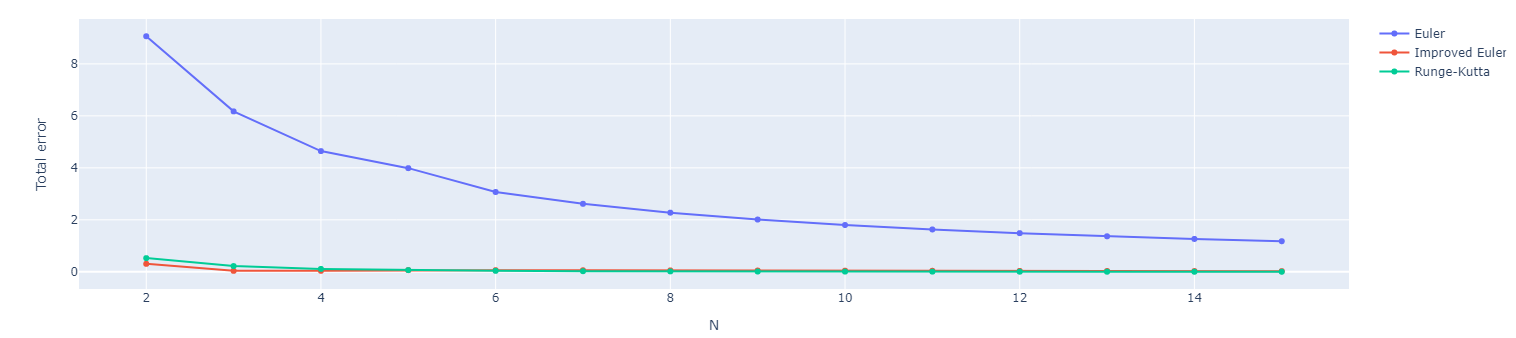
\includegraphics[width=1\linewidth]{total.png}
    % \caption{Graph of total approximation error}
    \centering The more points we use, the less total
approximation error.

\end{figure}

\begin{figure}[!h]
    \begin{center}
        \subsubsection*{Local truncation error}
    \end{center}
    \centering
        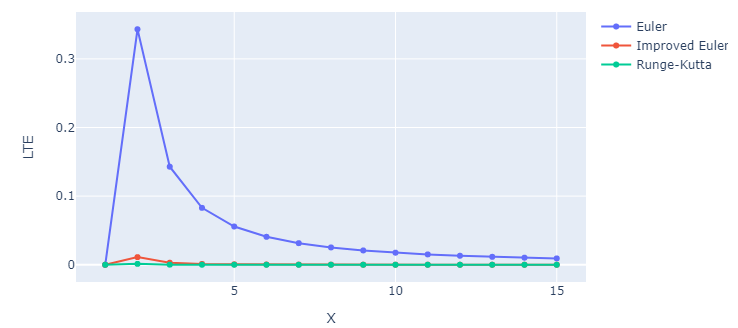
\includegraphics[width=0.8\linewidth]{lte.png}
    % \caption{Graph of local truncation error}
\end{figure}



\begin{figure}[!h]
    \begin{center}
        \subsubsection*{Global truncation error}
    \end{center}
    \centering
        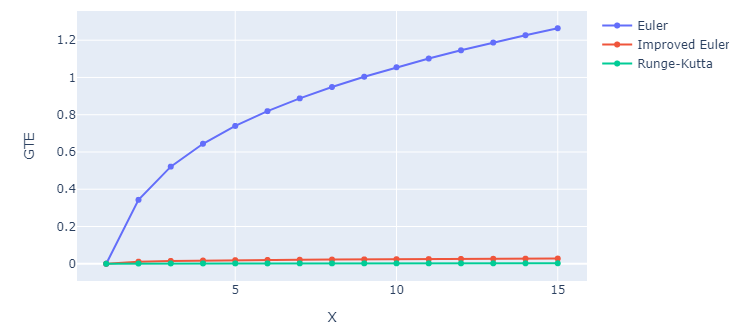
\includegraphics[width=0.8\linewidth]{gte.png}
    % \caption{Graph of global truncation error}
\end{figure}


\clearpage


\begin{center}
\subsection*{Tables}
\subsubsection*{Solutions}
        \resizebox{\textwidth}{!}{%
    \csvautotabular{dataframe.csv}
    %
    }
\end{center}


\begin{center}
\subsubsection*{Local and global truncation errors}

        \resizebox{\textwidth}{!}{%
    \csvautotabular{dataframe-errors.csv}
    %
    }
\end{center}

\begin{center}
\subsubsection*{Total errors}

        \resizebox{\textwidth}{!}{%
    \csvautotabular{total-errors.csv}
    %
    }
\end{center}

\begin{figure}[!h]
    \begin{center}
        \section*{UML diagram}
    \end{center}
    \centering
        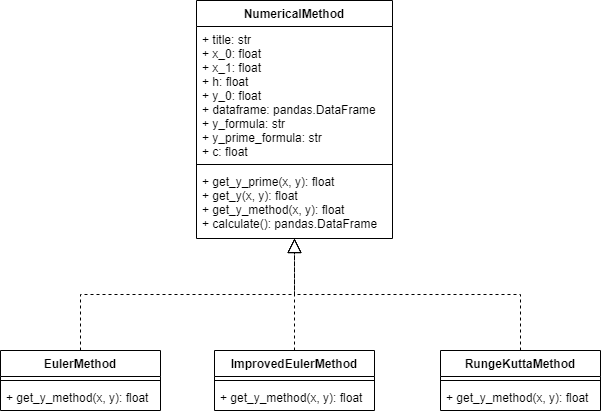
\includegraphics[width=1\linewidth]{uml.png}
    % \caption{Unified Modeling Language diagram}
\end{figure}

\begin{figure}[!h]
    \begin{center}
        \section*{Toggle callback graph}
    \end{center}
    \centering
        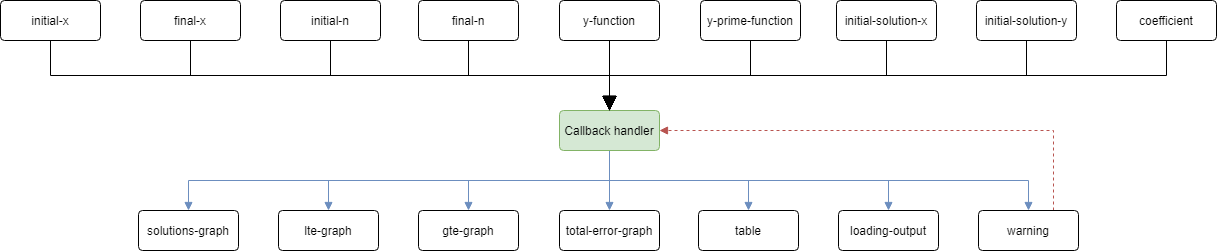
\includegraphics[width=1\linewidth]{callback.png}
    % \caption{Unified Modeling Language diagram}
\end{figure}

\end{document}
